
\section{JPEG Image Compression (ps6g08)}

\subsection{Introduction}
The images obtained from a camera will generally be in the JPEG image format
according to the 
EXIF (Exchangeable image file format for digital still cameras)
 (Exif Version 2.2).\cite{exif_std} 
JPEG is a form of image compression standard named after its developers, 
the Joint Photographic Experts Group. \cite{winzip_jpeg_compression}
This section will provide a quick overview of the JPEG image compression algorithm
and attempt to explain the information available by
analysing the JPEG file structure.

\subsection{JPEG Compression Process}

%%---------------------------------------
%%TO BE MOVED AND REFERENCED
%%---------------------------------------
\subsubsection{Colour Space Conversion (May be moved)(ps6g08)}
\label{sec:colour_space_conversion}
Initially, all image information is defined using the RGB colour model.
This means that each pixel's colour is defined by three values according to the RGB colour model. 
In this additive model, the pixel's colour is determined by a sum of red, green, and blue light. 
If each value for R, G, and B is represented with a single byte, 
this means that each pixel in an image has 3 bytes associated to it, so 
an image with $\mathbf{n}$ pixels would contain $\mathbf{3*n}$ bytes worth of information. 
For a 640x480 image, this means we have 921,600 bytes of information to send through.

Instead of storing all the image data using the RGB colour model, 
the JPEG file compresses the image data using chroma sub-sampling 
without losing any information that the human eye can discern. 
The image is put into  a luma-chrominance color space. In this form, the color of a pixel is described by two values, 
one (\emph{luma}) which describing its \emph{luminance} (brightness), and 
one (\emph{chrominance}) which describes its colour 
(represented using two components Cb and Cr).
These values are nonlinear representations
of the actual luminance and chrominance values.\cite{kerr_chroma_subsampling}

Although this also seperates a single pixel into three values like the RBG colour model, 
it allows for a more compact file due to the fact that the luma and chroma samples 
are not equally discerned by the human eye. 
In the RGB colour model, all three values must be taken at the same resolution in order to display the colour of one pixel. 
Lowering the resolution in this colour space quickly reduces the quality of an image. 

Chroma subsampling, or the YCbCr colour model, takes advantage of the fact that the human eye 
more easily distinguishes subtle differences in luminance than colour. \cite{kerr_chroma_subsampling} 
Therefore, by supporting different levels of resolution for the chroma and luma values, 
it is possible to lower the amount of information stored
 within an image which appears identical to the uncompressed image to human eye.

As an example, consider a 4x4 pixel image. 
Using the RGB colour model, the image would be represented with 48 bytes, 3 bytes for each pixel. 
With chroma subsampling, we can group 2 or 4 pixels together to form a \emph{chrominance pixel}. 
All the original image pixels in this new ``pixel'' would still be associated with a luma value (Y), but 
they would all share the same chrominance information (Cb and Cr). 
This means an image with $\mathbf{n}$ pixels would 
now contain $\mathbf{n+2n/c}$ bytes worth of information, where 
c is the size (in image pixels) of the chrominance pixel. 
In this example, using a resolution of 2 adjacent pixels 
gives us 32 byte and using a resolution of 2x2 pixel blocks 
gives us 24 bytes.

Commonly used chrominance subsampling patterns are designated as 
a string of 3 integers separated by colons. 
The relationship among the integers denotes 
the degree of vertical and horizontal subsampling.
The first integer is usually 4 and represents the 
now standard luma horizontal sampling rate. 
The second digit specifies the horizontal subsampling of 
both Cb and Cr with respect to luma.\cite{poynton_chroma_subsampling}.

If the third digit is the same as the second,
this denotes that there is no vertical subsampling.
If the third digit is zero, 2:1 vertical subsampling
for both Cb and Cr is indicated. This strange notation
is due to the invention of this notation
predating the concept of vertical subsampling.\cite{poynton_chroma_subsampling}.

The figure below compares 5 subsampling patterns used against a 2x2 pixel image.

\begin{figure}[!hbtp]
\begin{center}
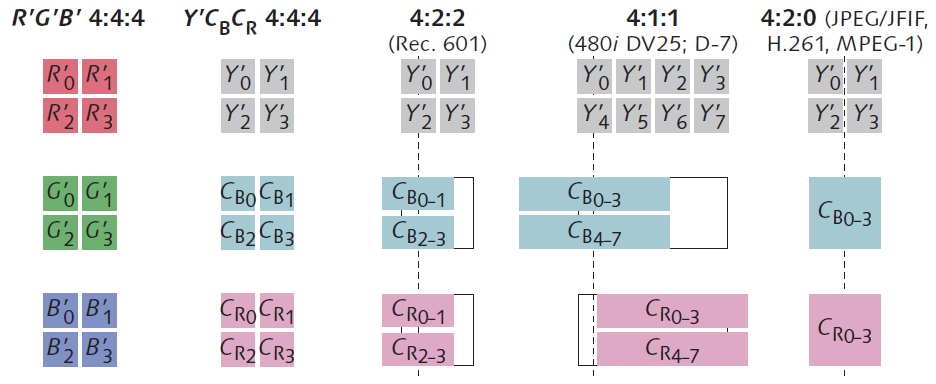
\includegraphics[scale=0.5]{figures/chromasub.png} 
\end{center}
\caption{Different chroma subsampling schemes for a 2x2 pixel colour image.\label{chroma_examples}\cite{poynton_chroma_subsampling}}
\end{figure}

%%---------------------------------------
%% END MOVED PART
%%---------------------------------------

The JPEG compression algorithm uses 8 
stages to compress an image: \cite{hass_impulse_jpeg}

\subsubsection{Colour Space Conversion}
The image undergoes chroma subsampling from the 
RGB colour model to a 4:2:2 or a 4:2:0 YCbCr colour model. 
Both subsampling patterns are approved by the
EXIF (Exchangeable image file format for digital still cameras)
and the pattern used is dependant on the camera's specifications. 
(see section \ref{sec:colour_space_conversion})

\subsubsection{Block Segmentation}
The image is then separated into 8x8 or 16x16 pixel blocks,
called MCUs (Minimum Coded Unit) 
depending on whether the image has been chroma
subsampled to a 4:2:2 or 4:2:0 model respectively. \cite{exif_std}

\subsubsection{Discrete Cosine Transform}
The image is transformed from a spatial domain 
representation to a frequency domain representation
using the Discrete Cosine Transform. \cite{hass_impulse_jpeg}
%%
%% REFERENCE TO DCT PART
%%(see section \ref{sec:jpegmanipulation})

\subsubsection{Quantization}
Using the wave equations from the DCT step,
the algorithm sorts them from low-frequency
components (gradual colour changes) to 
high-frequency components (sudden colour changes),
from the top left to the bottom right corner of the image.
The algorithm discards the high-frequency details
due to the human eye not recognizing them as
well as low-frequency details. This is down through 
division of all DCT wave equation 
coefficients using a quantization table and
then rounding the result to the nearest integer.
This quantization table differs between
the majority of digital cameras and 
software packages.\cite{hass_impulse_jpeg}

\subsubsection{Zigzag Scan}
The matrix obtained through quantization is
then re-ordered from the top-left corner into a 
64-element vector in a zig-zag pattern.
This is done to ensure that the high-frequency
components which are most likely to round to
zero after quantization, make up the lower
right hand part of the matrix.\cite{hass_impulse_jpeg}

\subsubsection{DPCM on DC components}
DPCM is known as Differential Pulse
Code Modulation. It is the process of
calculating the block-to-block average difference
of the DC components across the entire MCU block
and encoding the average as a change from the 
previous block's value.\cite{hass_impulse_jpeg}

\subsubsection{RLE on AC components}
RLE is known as Run Length Encoding. It is the process of
storing each value of the AC components of the
64-element vector with the number of zeros
preceding it for the purposes of the final stage.\cite{hass_impulse_jpeg}

\subsubsection{Entropy Coding/ Huffman Coding}
Finally, a dictionary representing commonly used value strings with
shorter code is created. Common string and patterns
are represented by short codes while less frequently
used strings are represented with longer codes.
%%
%% REFERENCE TO MICHAEL'S HT PART
%%(see section \ref{sec:jpegmanipulation})

\subsection{JPEG Structure}
A JPEG file can be separated into two main parts. 
The first part of the JPEG file is composed of segments containing information concerning 
various properties of the image which must be read in order to recover the image from its compressed form. 
The number of segments within one JPEG file varies from picture to picture.
The second part contains the entropy-encoded image data, which can be decoded using the information provided from the headers of the file.  

\subsubsection{JPEG Segments}
The JPEG headers are capable of storing most of the metadata related to an image, not all of which is necessary for the decompression of the image. 
The following headers are those which contain all the information necessary for 
a successful decompression of the JPEG image, as well as those which can be found in all JPEG images.
The SOI (Start Of Image) and APP (JFIF application) segments are recorded first, in that order.
These segments are followed by the DQT (Define Quantization Table(s)), DHT (Define Huffman Table(s)), and SOF (Start Of Frame) segments,
in any order depending on the image. The SOS (Start Of Scan) and entropy- encoded data are 
stored afterwards and the image ends with the EOI (End Of Image) segment.

The following table details some important segments which are necessary for the image
to be properly displayed: \cite{exif_std}

\begin{table}[!hbtp]
	\caption{JPEG File Layout}
	\centering
	\begin{tabular}{ | p{1.5cm} | p{3cm} | p{2cm} | p{2.8cm} | }
	\hline
	\textbf{Segment Name} & \textbf{Marker Name} & 
	\textbf{Marker Code} & \textbf{Description} \\ \hline
	SOI & Start Of Image & 0xD8 & Start of compressed image data\\ \hline
	APP\emph{n} & Application Segment \emph{n} & 0xE\emph{n} & Exif application information segment\\ \hline
	DQT & Define Quantization Table(s) & 0xDB & Quantization table definition.\\ \hline
	DHT & Define Huffman Table(s) & 0xC4 & Huffman table definition.\\ \hline
	SOF & Start Of Frame & 0xC0 & Frame parameter data\\ \hline
	SOS & Start Of Scan & 0xDA & Scan parameter data\\ \hline
	\end{tabular}
\end{table}

The following tables show important compression contents from the relevant JPEG file segments.

%% MOVE TO APPENDIX
%% \label{sec: jpeg_segment_content}
%%
\newpage

\textbf{SOF0: Start Of Frame (0xc0):}

\begin{table}[!hbtp]
	\caption{SOF0 Marker Content}
	\centering
	\begin{tabular}{ | p{2cm} | p{1.5cm} | p{4cm} | }
	\hline
	\textbf{Field} & \textbf{Size} & \textbf{Comments} \\ \hline
	Length & 2 bytes & Equal to 8 + the number of components used in the colour scheme * 3\\ \hline
	Data precision & 1 byte & Value shown in bits/sample. Usually 8 signifying bytes.\\ \hline
	Image height  & 2 bytes & ----\\ \hline
	Image width  & 2 bytes & ----\\ \hline
	Number of components & 1 byte & indicates the number of components used  in the colour scheme\\ \hline
	Component information & 3 bytes / component & See component information table below.\\ \hline
	\end{tabular}
\end{table}

\begin{table}[!hbtp]
	\caption{SOF Component Information}
	\centering
	\begin{tabular}{ | p{2cm} | p{4cm} | }
	\hline
	\textbf{Byte Number} &  \textbf{Information} \\ \hline
	1 & Component ID (1 = Y, 2 = Cb, 3 = Cr, 4 = I, 5 = Q)\\ \hline
	2 & Sampling factors (bits 0\ldots3 : vertical, bits 4\ldots7 horizontal)\\ \hline
	3 & Quantization table number\\ \hline
	\end{tabular}
\end{table}

\newpage

\textbf{DHT: Define Huffman Table(s) (0xc4):}

\begin{table}[!hbtp]
	\caption{DHT Marker Content}
	\centering
	\begin{tabular}{ | p{2cm} | p{1.5cm} | p{4cm} | }
	\hline
	\textbf{Field} & \textbf{Size} & \textbf{Comments} \\ \hline
	Length & 2 bytes & ----\\ \hline
	HT Information & 1 byte & See HT Information table below\\ \hline
	Number of Symbols  & 16 bytes & Number of symbols with codes of length 1\ldots16.
	The sum of these values (\emph{n})must be $\le$ 256\\ \hline
	Symbols  & \emph{n} bytes & Symbols of the HT in order of increasing code length\\ \hline
	\end{tabular}
\end{table}

\begin{table}[!hbtp]
	\caption{HT Information Byte Content}
	\centering
	\begin{tabular}{ | p{2cm} | p{4cm} | }
	\hline
	\textbf{Bit} &  \textbf{Information} \\ \hline
	0\ldots3 & ID number of HT\\ \hline
	4 & type of HT, 0 = DC table, 1 = AC table\\ \hline
	5\ldots7 & Unused\\ \hline
	\end{tabular}
\end{table}

\textbf{DQT: Define Quantization Table(s) (0xdb):}

\begin{table}[!hbtp]
	\caption{DQT Marker Content}
	\centering
	\begin{tabular}{ | p{2cm} | p{1.5cm} | p{4cm} | }
	\hline
	\textbf{Field} & \textbf{Size} & \textbf{Comments} \\ \hline
	Length & 2 bytes & ----\\ \hline
	QT Information & 1 byte & See QT Information table below\\ \hline
	Bytes  & \emph{n} bytes & QT values. \emph{n} = 64 * (QT precision + 1) \\ \hline
	\end{tabular}
\end{table}

\begin{table}[!hbtp]
	\caption{QT Information Byte Content}
	\centering
	\begin{tabular}{ | p{2cm} | p{4cm} | }
	\hline
	\textbf{Bit} &  \textbf{Information} \\ \hline
	0\ldots3 & ID number of QT\\ \hline
	4\ldots7 & precision of QT (0 = 8 bit, else 16 bit)\\ \hline
	\end{tabular}
\end{table}

\newpage

\textbf{SOS: Start Of Scan (0xda):}

\begin{table}[!hbtp]
	\caption{SOS Marker Content}
	\centering
	\begin{tabular}{ | p{2cm} | p{1.5cm} | p{4cm} | }
	\hline
	\textbf{Field} & \textbf{Size} & \textbf{Comments} \\ \hline
	Length & 2 bytes & Equal to 6 + 2 * (number of components in scan)\\ \hline
	Number of components in scan & 1 byte & Within range 1 to 4\\ \hline
	Component information & 2 bytes / component & See component information table below.\\ \hline
	Ignorable Bytes & 3 bytes & Separates header information from entropy-encoded image data\\ \hline
	\end{tabular}
\end{table}

\begin{table}[!hbtp]
	\caption{SOS Component Information Content}
	\centering
	\begin{tabular}{ | p{2cm} | p{4cm} | }
	\hline
	\textbf{Byte Number} &  \textbf{Information} \\ \hline
	1 & Component ID (1 = Y, 2 = Cb, 3 = Cr, 4 = I, 5 = Q)\\ \hline
	2 & HT to use (bits 0\ldots3 : AC Table ID, bits 4\ldots7 DC Table ID)\\ \hline
	\end{tabular}
\end{table}

\subsubsection{Entropy-encoded image data}

The image data is received chrominance pixel by chrominance pixel. 
The first bytes received are the luma values of the individual image pixels. 
In the case of JPEG images, they are received from left to right, top to bottom, moving horizontally before vertically. 
The luma values are then followed by the Cb and Cr values of the top-left pixel, in that order. 
After all the data for a single chrominance pixel has been sent (6 bytes) those of the next chrominance pixel are sent in the same format, 
read in the same order as the image pixels within one chrominance pixel. This continues until the EOI marker is found.
